\section{Testy}

TODO -- proszę uzupełnić.

Wyniki profilowania algorytmu CHARM znajdują się na Rys. \ref{charm:profil}. Tak jak można było się spodziewać, większość czasu program spędził w głównej metodzie algorytmu. Można zauważyć, że aż 10\% czasu procesora zostało zużyte na wyliczanie funkcji skrótu obiektów. Wynika to z tego, że w algorytmie występuje bardzo dużo porównywania zbiorów transakcji, w których występują poszukiwane zbiory częste. Jako, że najszybsze wyszukiwanie w tego typu warunkach gwarantowały kolekcje \emph{HashSet}, to one zostały wykorzystane w tych kluczowych miejscach. Na dole wykresu widać także, że wykorzystanie 13\% czasu procesora związane było z obsługą wielowątkowości. Pomimo nie napisania żadnego specjalnego kodu do obsługi wielu wątków dzięki wykorzystaniu mechanizmu \emph{parallelStream}, który pojawił się w Java 8, w bardzo prosty sposób można zrównoleglić niektóre operacje na kolekcjach, co zostało wykorzystane w projekcie.

\begin{figure}
\caption{Wyniki profilowania algorytmu CHARM}
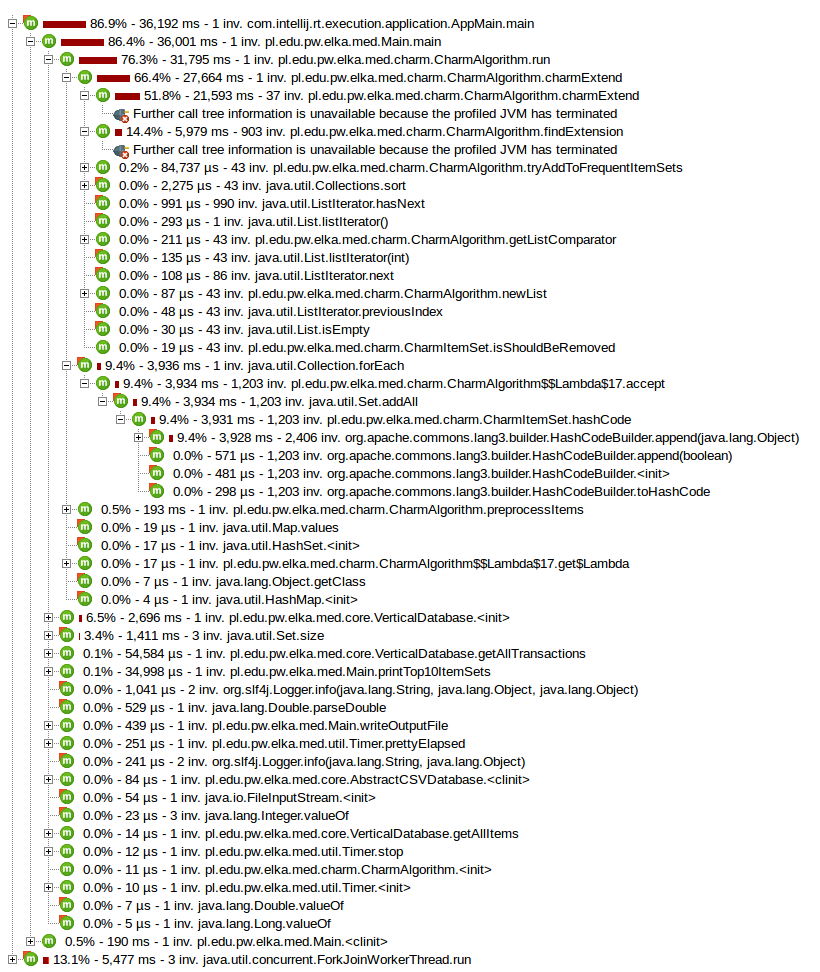
\includegraphics[width=17cm]{res/charm-profi.png}
\label{charm:profil}
\end{figure}
